\documentclass[10pt]{beamer}
\usepackage[utf8]{inputenc}

\usepackage[absolute,overlay]{textpos}
\usepackage{graphicx}
\usepackage{listings}
\lstset{
  language=Python,
  basicstyle=\ttfamily\small,
  commentstyle=\color{gray},
  keywordstyle=\color{blue},
  stringstyle=\color{red},
  showstringspaces=false,
  numbers=left,
  numberstyle=\tiny,
  frame=single,
  breaklines=true,
}
\mode<presentation> {
\usetheme{boxes} % When headline is wanted use Dresden theme instead
\usecolortheme{seagull}
\logo{
\includegraphics[height=1.5cm]{ku_logo_dk}}
\setbeamertemplate{footline}[frame number]
% \setbeamertemplate{footline}{
%   \hspace{1em}
%   \hfill
%   \insertframenumber/\inserttotalframenumber
%   \vspace{1em}
%   \hspace{1em}
%   
\includegraphics[height=2cm]{ku_logo_dk}
%   \hspace{1em}
% }
\setbeamertemplate{navigation symbols}{}
\setbeamertemplate{itemize items}[square]
}


%----------------------------------------------------------------------------------------
%	TITLE PAGE
%----------------------------------------------------------------------------------------

\title[Kickstart-kursus] % bottom of every slide
  {Kickstart-kursus i programmering 23 dag 2} % title page

\author{\footnotesize{Daniel Spikol} \\
          \footnotesize{\texttt{ds@di.ku.dk}}}

\institute {DIKU \\ Københavns Universitet}

\date[15. august 2023]{15 august 2023}

\begin{document}
\begin{frame}[plain]
\titlepage
\end{frame}


%%----------------------------------------------%%

\begin{frame}
   \frametitle{Recap from Yesterday}
   	\begin{itemize}
	\item Marshmallow Challenge - constant prototyping as a problem-solving method
	\item Coordinate System 
	\item Drawing with Processing
	\item Variables
	\item Functions maybe...
	\end{itemize}
\end{frame}

%%----------------------------------------------%%

\begin{frame}
\frametitle{Todays Plan - IFOs}
\begin{itemize}
\item Let's dig into basic Python and Functions
\item Making some Animations
\item Exploring Pair Programming
\end{itemize}
\end{frame}


%%----------------------------------------------%%
%% Basic Structure of Python Processing
%%----------------------------------------------%%

\begin{frame}{The Python of Python}
    	 
\includegraphics[height=6cm]{images/MPFC-logo}
\end{frame}

%%----------------------------------------------%%

\begin{frame}{What the heck is Python}
    \begin{itemize}
	\item A high-level, interpreted programming language known for its simplicity and readability.
	\item Supports multiple programming paradigms: procedural, object-oriented, and functional.
	\item Extensive standard libraries and vast ecosystem of third-party packages.
	\item Used for web development, data analysis, artificial intelligence, scientific computing, and more.
	\item Guiding principle: "There should be one—and preferably only one—obvious way to do it." (From the Zen of Python)
\end{itemize}
\end{frame}

%%----------------------------------------------%%

\begin{frame}{Brief History of Python}
    \begin{itemize}
	\item Created by Guido van Rossum and first released in 1991.
	\item Named not after the snake, but after the British comedy series "Monty Python's Flying Circus", which Guido enjoyed.
	\item Python 2.0 (2000) introduced new features like garbage collection and Unicode support.
	\item Python 3.0 (2008) was a major overhaul fixing inconsistencies, focusing on removing duplicate constructs and modules.
	\item Python's popularity Continues growing due to its ease of learning and versatility, with a strong community support and a wealth of libraries and frameworks.
\end{itemize}
\end{frame}

%%----------------------------------------------%%
%% FUNCTIONS
%%----------------------------------------------%%
\begin{frame}[fragile]{What are Functions}{Basic}
	%\frametitle{What are Functions (Basic)}
	\begin{itemize}
		\item Writing a program is like writing a recipe. 
		\item Similar to how a recipe is a set of steps another person follows, a program is a set of steps the computer follows.
		\item A single recipe step might be “preheat the oven to 350 degrees” or “add 2 cups of flour”, and you might write each step on its line. 
		\item The other person then follows those steps in order, one after the other, to bake a cake.
	\end{itemize}
\begin{lstlisting}
preheat oven to 350 degrees
get a large bowl
add 2 cups of flour
add 1 cup of sugar
...
\end{lstlisting}	

\end{frame}

%%----------------------------------------------%%
\begin{frame}[fragile]{Functions in Programming} % Note the 'fragile' option; it's important for listings
\begin{itemize}
\item This is similar to how a computer program works. A program is a set of instructions that tells the computer to follow a series of steps. 
\item Each step is written on its line, and the computer follows the instructions individually.
\item A function is one of those steps. Calling a function gives the computer a single instruction that tells it to do one thing.
\end{itemize}
\end{frame}

%%----------------------------------------------%%
\begin{frame}[fragile]{Py. Processing}{Examples}
\begin{lstlisting}
def drawFish(fishX, fishY, eyeSize):
    # Krop
    fill(255, 157, 0)
    ellipse(fishX, fishY, 120, 75)
    
    # Finner
    fill(247, 222, 0)
    triangle(fishX-60, fishY, fishX-90, fishY-30, fishX-90, fishY+30)
    triangle(fishX+10, fishY+10, fishX-20, fishY, fishX-20, fishY+25)

    # Eye
    fill(0, 0, 0)
    ellipse(fishX + 30, fishY-10, eyeSize, eyeSize)
    fill(255, 255, 255)
    ellipse(fishX + 32, fishY-10, 5, 5)

\end{lstlisting}	
\end{frame}

%%----------------------------------------------%%

\begin{frame}[fragile]{Python Syntax}
Python is a programming language that follows a simple, clean, and readable format. Here's a basic breakdown:
\begin{itemize}
\item \textbf{Indentation:} Instead of using braces \{\} like many other languages, Python uses indentation (spaces or tabs) to denote code blocks. The amount of indentation should be consistent throughout a block.
\begin{lstlisting}
def say_hello():
    print("Hello!")
\end{lstlisting}
\item \textbf{Colons:} Statements that introduce a new block, like if, for, def (for defining functions), end with a colon :
\begin{lstlisting}
def drawStones(stonesX):
    fill(88, 42, 26)
\end{lstlisting}
\item \textbf{Comments:} Any line that starts with a \# is a comment, meaning Python ignores it. It's for the programmer to write notes.
\begin{lstlisting}
# This is a comment
print("This is not a comment")
\end{lstlisting}
\end{itemize}
\end{frame}


%%----------------------------------------------%%

\begin{frame}{Basic Structure for Processing}
    	 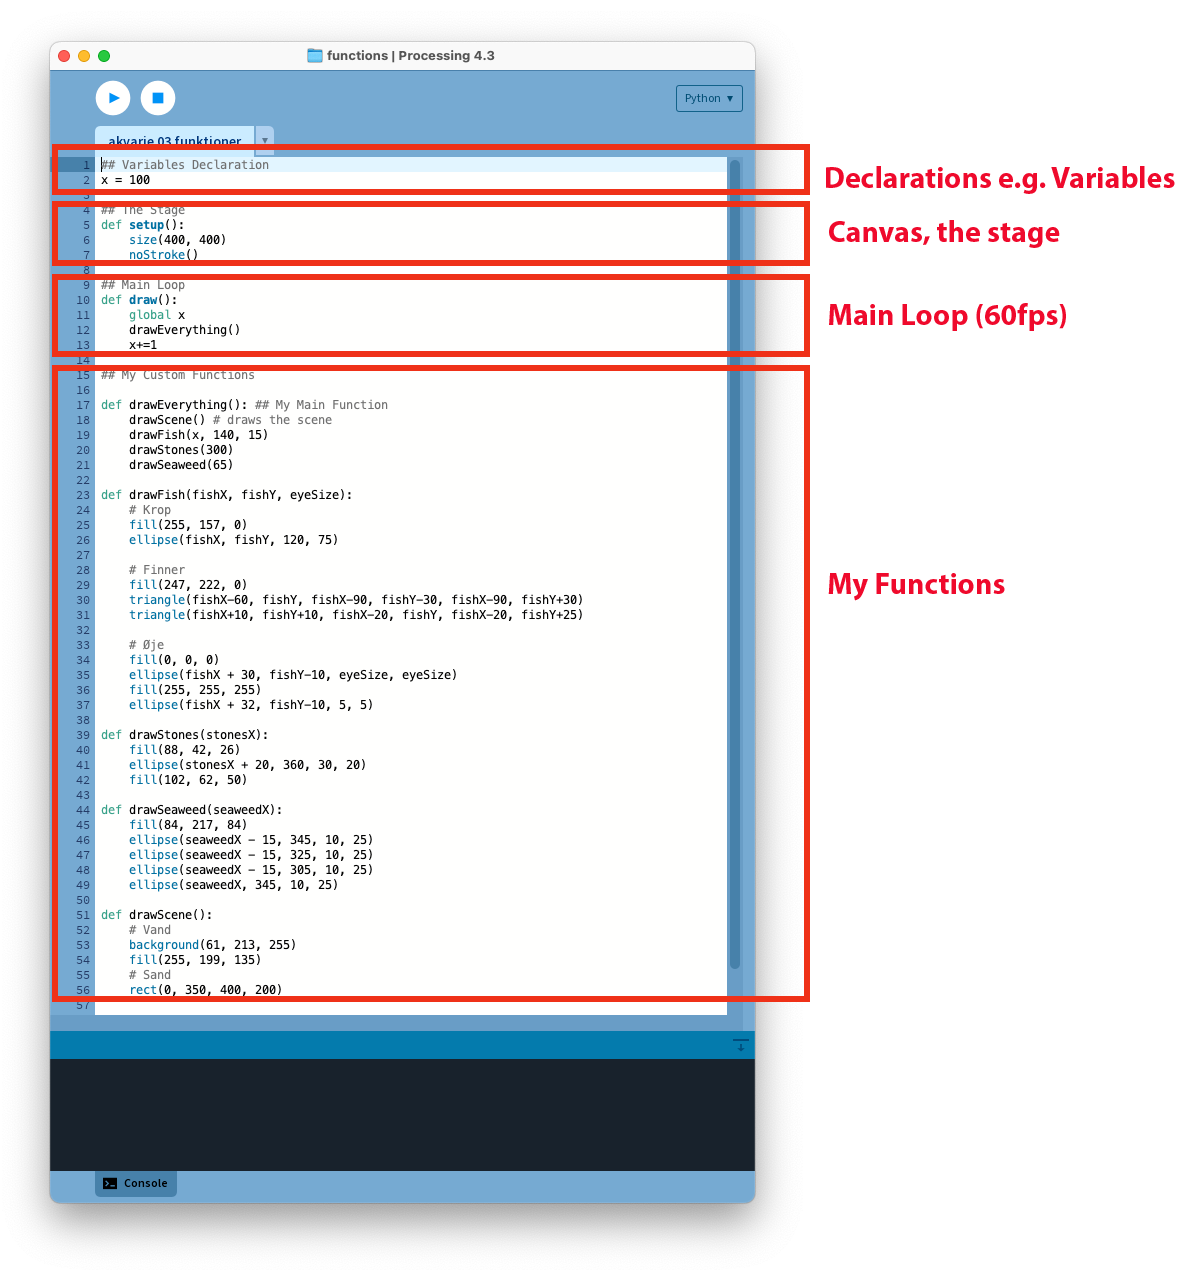
\includegraphics[height=8cm]{images/process}
\end{frame}

%%----------------------------------------------%%

\begin{frame}{Debugging Strategies}
    	 \begin{enumerate}
\def\labelenumi{\arabic{enumi}.}
\item
  \textbf{Print Statements}:

  \begin{itemize}
  \item
    Sometimes, the simplest methods are the most effective. Use
    \texttt{print()} to display the values of variables, the flow of the
    program, or to check if a specific part of the code is being
    executed. This can quickly help you locate where things might be
    going wrong.
  \end{itemize}
\item
  \textbf{Error Messages}:

  \begin{itemize}
  \item
    Always read error messages in the Processing console. They can give
    you precise information on what went wrong and where. For instance,
    a \texttt{NullPointerException} might indicate you're trying to use
    an object that hasn't been initialized.
  \end{itemize}
\item
  \textbf{Commenting Out}:

  \begin{itemize}
  \item
    If you're unsure which part of your code is causing the problem, try
    commenting out sections of it to isolate the problematic area. You
    can gradually uncomment sections to narrow down the issue.
  \end{itemize}
\item
  \textbf{Visual Feedback}:

  \begin{itemize}
  \item
    Since Processing is a graphical environment, use visual feedback to
    your advantage. For example, change colors, draw borders, or use
    simple shapes to visually represent the flow of logic or the state
    of specific variables.
  \end{itemize}
\end{enumerate}
\end{frame}

%%----------------------------------------------%%

\begin{frame}{Meta Debugging Strategies}
    	 \begin{enumerate}
\def\labelenumi{\arabic{enumi}.}
\item
  \textbf{Break Down the Problem}:

  \begin{itemize}
  \item
    If you have a complex piece of code that isn't working, break it
    down into smaller, more manageable chunks. Test each chunk
    independently to ensure it works as expected before integrating it
    back into the larger codebase.
  \end{itemize}
\item
  \textbf{Check for Common Mistakes}:

  \begin{itemize}
  \item
    In the context of Processing, this might mean:

    \begin{itemize}
    \item
      Make sure \texttt{setup()} and \texttt{draw()} functions are
      correctly defined.
    \item
      Ensuring that you're using the right coordinates or dimensions for
      shapes.
    \item
      Verifying that image or data files are in the correct directory
      and are being loaded properly.
    \end{itemize}
  \end{itemize}
\end{enumerate}
\end{frame}

%%----------------------------------------------%%

\begin{frame}{Some Toolsl in the PDE}
    	 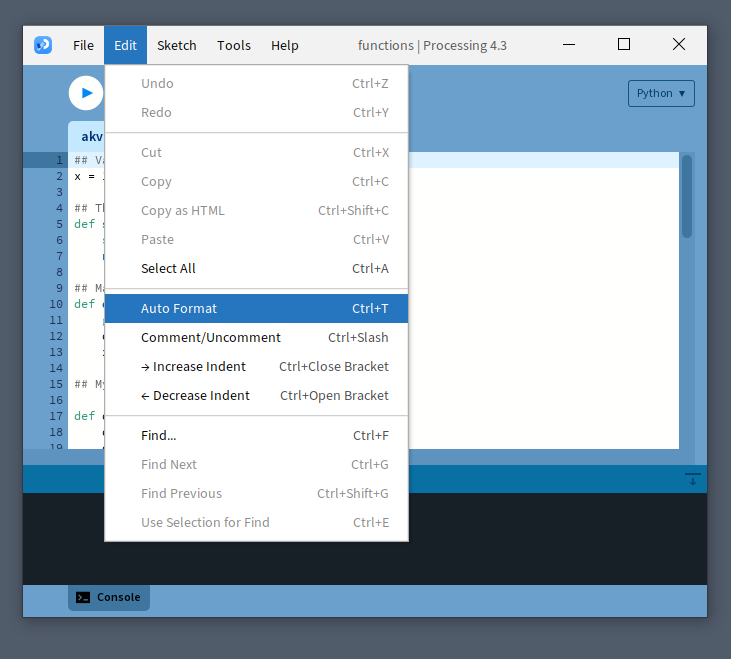
\includegraphics[height=7cm]{images/auto_for}
\end{frame}


% parts of the programming
% Structure and Commenting
% Identation
% Debugging
% Functions
% Variables - scoping
% Mouse and Keyboard

%%----------------------------------------------%%
%% PAIR PROGRAMMING
%%----------------------------------------------%%



\begin{frame}
   \frametitle{Pair Programming - Hello Friend!}
   	 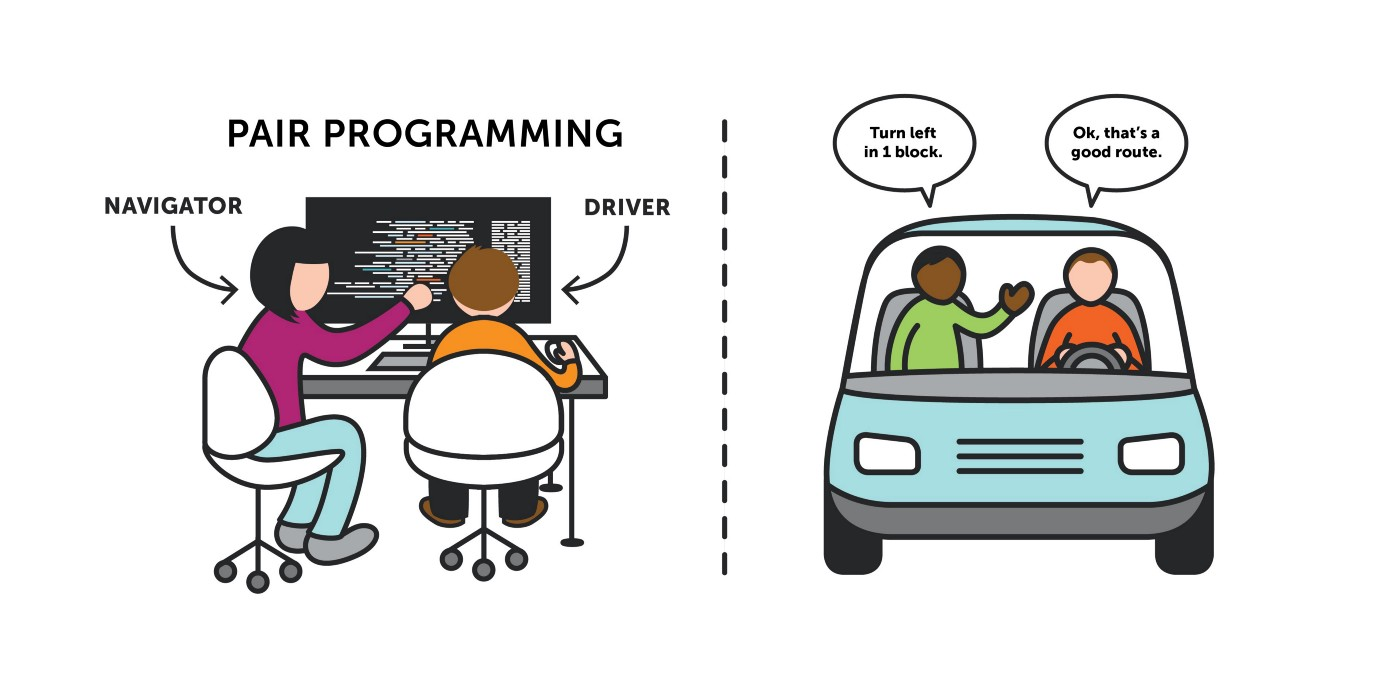
\includegraphics[height=8cm]{images/pairprog}
\end{frame}

%%----------------------------------------------%%

\begin{frame}
   \frametitle{Two heads are better than one}
   \framesubtitle{Pair programming}

  \begin{itemize}
   \item Couple of programmers develop higher-quality software
   \item Slightly longer development time, but much less time spent on
     find errors afterwards.
   \item Cozier and more fun than working alone.
% \item More enjoyable than working alone, pair programmers are happier programmers
% \item Creates Closer social connections
   \item Improved knowledge sharing between the programmers, less time spent
     on coordination %Improved knowledge transfer
   \item Increased learning (and that's why you're here, isn't it?), you take turns
     a way to teach each other
     % \item Enhanced learning
     % \item Taking turns being the teacher
   \item Otherwise, unspoken knowledge and habits are exchanged
% \item Unspoken skills and habits are exchanged
   \end{itemize}
\end{frame}

%%----------------------------------------------%%

\begin{frame}
   \frametitle{Pair programming in practice}

  Two programmers, one computer
     \begin{itemize}
     \item Driver - has hands on the steering wheel (keyboard)
       and eyes on the road (screen)
     \item Navigator - focuses on the destination and
       how we get there
     \end{itemize}
~
Rules
\begin{itemize}
   \item You must not be bossy towards your partner
   \item The navigator must not touch the mouse or keyboard
   \item The driver must not ignore the navigator
   \item You must switch roles often (e.g. every 20 minutes)
   \item Try to keep a conversation going
   \end{itemize}
\end{frame}
 
%%----------------------------------------------%%

\begin{frame}
   \frametitle{Conversations between driver and navigator}
     \begin{itemize}
   \item Good pair programming is not without communication and talk.
   \item Talk together as a pair about what is happening
     on the screen.
   \item Reflect on what you have done and where you are going.
   \item The driver tells what they are doing and what is happening.
   \item The navigator makes comments, ensures they are running
     with the right thing and tells what they have to do now and later.
   \end{itemize}
   ~
   Examples:
   \begin{itemize}
   \item Driver: ``Now we create a new function to draw a sunflower.''
   \item Driver: ``Now we just test whether XYZ works before we continue.''
   \item Navigator: ``How can you do that?''
   \item Navigator: ``Can you explain what you're doing?''
   \end{itemize}
\end{frame}


%%----------------------------------------------%%
\begin{frame}{Recap}
    	 \begin{itemize}
	 \item Python Syntax and Structure
	 \item Functions and Animations
	 \item Debugging
	 \item Pair Programming
	\end{itemize}
	 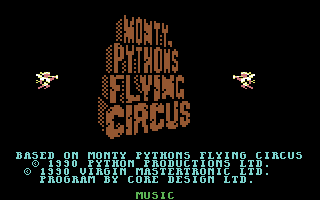
\includegraphics[height=5cm]{images/mpfc_game}
\end{frame}

%%----------------------------------------------%%
\begin{frame}{Wednesday}
    	 \begin{itemize}
	 \item Conditionals
	 \item more input with keys and mouse
	 \item Finite State Machines?
	 \item Brainstorming Ideas for your Projects!
	\end{itemize}
	 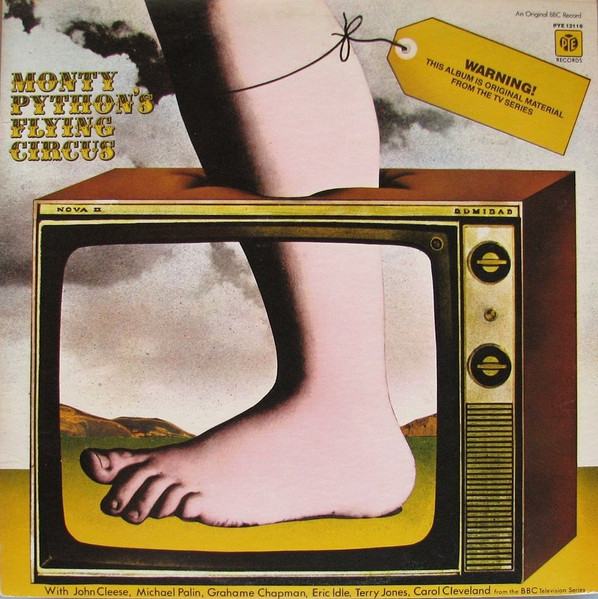
\includegraphics[height=6cm]{images/tomorrow_mpfc}
\end{frame}

%%----------------------------------------------%%

\end{document}